\documentclass[bachelor, och, labwork]{shiza}
% параметр - тип обучения - одно из значений:
%    spec     - специальность
%    bachelor - бакалавриат (по умолчанию)
%    master   - магистратура
% параметр - форма обучения - одно из значений:
%    och   - очное (по умолчанию)
%    zaoch - заочное
% параметр - тип работы - одно из значений:
%    referat    - реферат
%    coursework - курсовая работа (по умолчанию)
%    diploma    - дипломная работа
%    pract      - отчет по практике
% параметр - включение шрифта
%    times    - включение шрифта Times New Roman (если установлен)
%               по умолчанию выключен
\usepackage{subfigure}
\usepackage{tikz,pgfplots}
\pgfplotsset{compat=1.5}
\usepackage{float}

%\usepackage{titlesec}
\setcounter{secnumdepth}{4}
%\titleformat{\paragraph}
%{\normalfont\normalsize}{\theparagraph}{1em}{}
%\titlespacing*{\paragraph}
%{35.5pt}{3.25ex plus 1ex minus .2ex}{1.5ex plus .2ex}

\titleformat{\paragraph}[block]
{\hspace{1.25cm}\normalfont}
{\theparagraph}{1ex}{}
\titlespacing{\paragraph}
{0cm}{2ex plus 1ex minus .2ex}{.4ex plus.2ex}

% --------------------------------------------------------------------------%


\usepackage[T2A]{fontenc}
\usepackage[utf8]{inputenc}
\usepackage{graphicx}
\graphicspath{ {./images/} }
\usepackage{tempora}

\usepackage[sort,compress]{cite}
\usepackage{amsmath}
\usepackage{amssymb}
\usepackage{amsthm}
\usepackage{fancyvrb}
\usepackage{listings}
\usepackage{listingsutf8}
\usepackage{longtable}
\usepackage{array}
\usepackage[english,russian]{babel}

\usepackage[colorlinks=false]{hyperref}
\usepackage{url}

\usepackage{underscore}
\usepackage{setspace}
\usepackage{indentfirst} 
\usepackage{mathtools}
\usepackage{amsfonts}
\usepackage{enumitem}
\usepackage{tikz}
\usepackage{verbatim}
\usepackage{minted}

\newcommand{\eqdef}{\stackrel {\rm def}{=}}
\newcommand{\specialcell}[2][c]{%
\begin{tabular}[#1]{@{}c@{}}#2\end{tabular}}

\renewcommand\theFancyVerbLine{\small\arabic{FancyVerbLine}}

\newtheorem{lem}{Лемма}

\begin{document}

% Кафедра (в родительном падеже)
\chair{теоретических основ компьютерной безопасности и криптографии}

% Тема работы
\title{приближенные вычисления: задача о разбиении на равные части}

% Курс
\course{3}

% Группа
\group{331}

% Факультет (в родительном падеже) (по умолчанию "факультета КНиИТ")
\department{факультета КНиИТ}

% Специальность/направление код - наименование
%\napravlenie{09.03.04 "--- Программная инженерия}
%\napravlenie{010500 "--- Математическое обеспечение и администрирование информационных систем}
%\napravlenie{230100 "--- Информатика и вычислительная техника}
%\napravlenie{231000 "--- Программная инженерия}
\napravlenie{10.05.01 "--- Компьютерная безопасность}

% Для студентки. Для работы студента следующая команда не нужна.
% \studenttitle{Студентки}

% Фамилия, имя, отчество в родительном падеже
\author{Токарева Никиты Сергеевича}

% Заведующий кафедрой
% \chtitle{} % степень, звание
% \chname{}

%Научный руководитель (для реферата преподаватель проверяющий работу)
\satitle{доцент} %должность, степень, звание
\saname{А. Н. Гамова}

% Руководитель практики от организации (только для практики,
% для остальных типов работ не используется)
% \patitle{к.ф.-м.н.}
% \paname{С.~В.~Миронов}

% Семестр (только для практики, для остальных
% типов работ не используется)
%\term{8}

% Наименование практики (только для практики, для остальных
% типов работ не используется)
%\practtype{преддипломная}

% Продолжительность практики (количество недель) (только для практики,
% для остальных типов работ не используется)
%\duration{4}

% Даты начала и окончания практики (только для практики, для остальных
% типов работ не используется)
%\practStart{30.04.2019}
%\practFinish{27.05.2019}

% Год выполнения отчета
\date{2022}

\maketitle

% Включение нумерации рисунков, формул и таблиц по разделам
% (по умолчанию - нумерация сквозная)
% (допускается оба вида нумерации)
% \secNumbering

%-------------------------------------------------------------------------------------------

\tableofcontents


\section{Разбиение множества на равные части}

Необходимо выполнить следующие задачи:

\begin{enumerate}
  \item Вычислить сумму $sum$ массива. Если сумма нечетная, не может быть двух подмножеств с одинаковой суммой, поэтому верните false;
  \item Если сумма элементов массива четная, вычислить $sum_{\frac{1}{2}} = sum / 2$ найти подмножество массива с суммой, равной $sum_{\frac{1}{2}}$.
\end{enumerate}

  Вычисление подмножества происходит следующим образом:

  \textit{Вход}: Конечное множество символов $S$ мощности $n$ и сумма $sum_{\frac{1}{2}}$.\\

  \textit{Выход}: Подмножества $A$ и $\overline{A}$ такие что $S = A \cup \overline{A}$.\\
  \begin{enumerate}
    \item Инициализировать переменную $cnt = sum_{\frac{1}{2}}$, создать список $list = [x_0, \dots , x_{n - 1}]$, где $x_i \in S$ ($1 \leq i < n$) и
    пустой список $partition = []$.
    \item Пока переменная $cnt != 0$ выполнять: $cnt = cnt - list[n - 1]$, добавить в $partition$ элемент $list[n - 1]$, $n = n - 1$.
    \item Может оказаться так, что $cnt$ станет меньше нуля. В таком случае вернуться к первому пункту. Если $cnt = 0$, то мы получили подмножество, 
    элементы которого находятся в $partition$.
    \item Далее найдем элементы множества $S \backslash partition$.  
  \end{enumerate}
  
  \section{Код программы, реализующий алгоритм}

  Далее представлена реализация данного алгоритма, написанная на языке $Python$.

  
  \inputminted[fontsize=\small]{Python}{code/set-partition.py}


  На рисунке 1 представлен результат работы алгоритма.

  \begin{figure}[H]
    \centering
    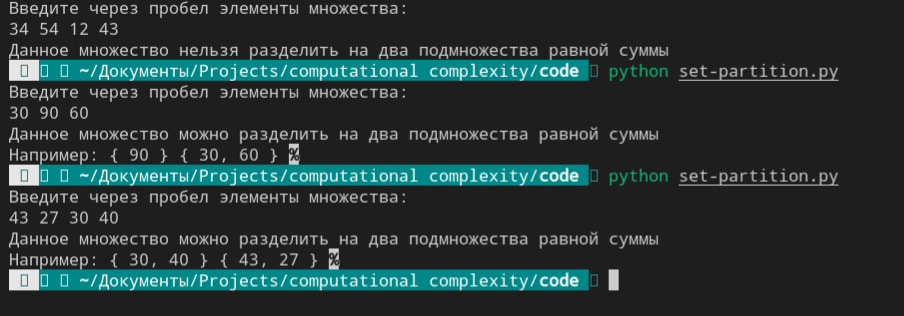
\includegraphics[width=0.8\textwidth]{img/5-1.png}
    \caption{Результат работы алгоритма}
  \end{figure}

  \textbf{Анализ алгоритма}

  Очевидно, что сложность данного алгоритма равна $O(2^n)$, так как в худшем случае это
  решение пробует две возможности (включить или исключить текущий элемент) для каждого элемента.

\conclusion

В данной лабораторной работе был рассмотрен алгоритм разбиения множества на подможества с одинаковыми суммами и был проведен анализ оценки его сложности.
Это послужило созданием её программной реализации, написанной на языке $Python$. 

\begin{thebibliography}{3}
  \bibitem{1}
  Статья <<Partition of the set>>  / [Электронный ресурс] URL: https://www.tutorialspoint.com/partitioning-of-a-set (дата обращения 02.05.2022), Яз. рус.
  \bibitem{2}
  Книга Томаса Кормена <<Алгоритмы>> / [Электронный ресурс] URL: https://e-maxx.ru/bookz/files/cormen.pdf (дата обращения 02.05.2022), Яз. рус.
\end{thebibliography}

\end{document}
